\begin{figure*}[t]
\centering
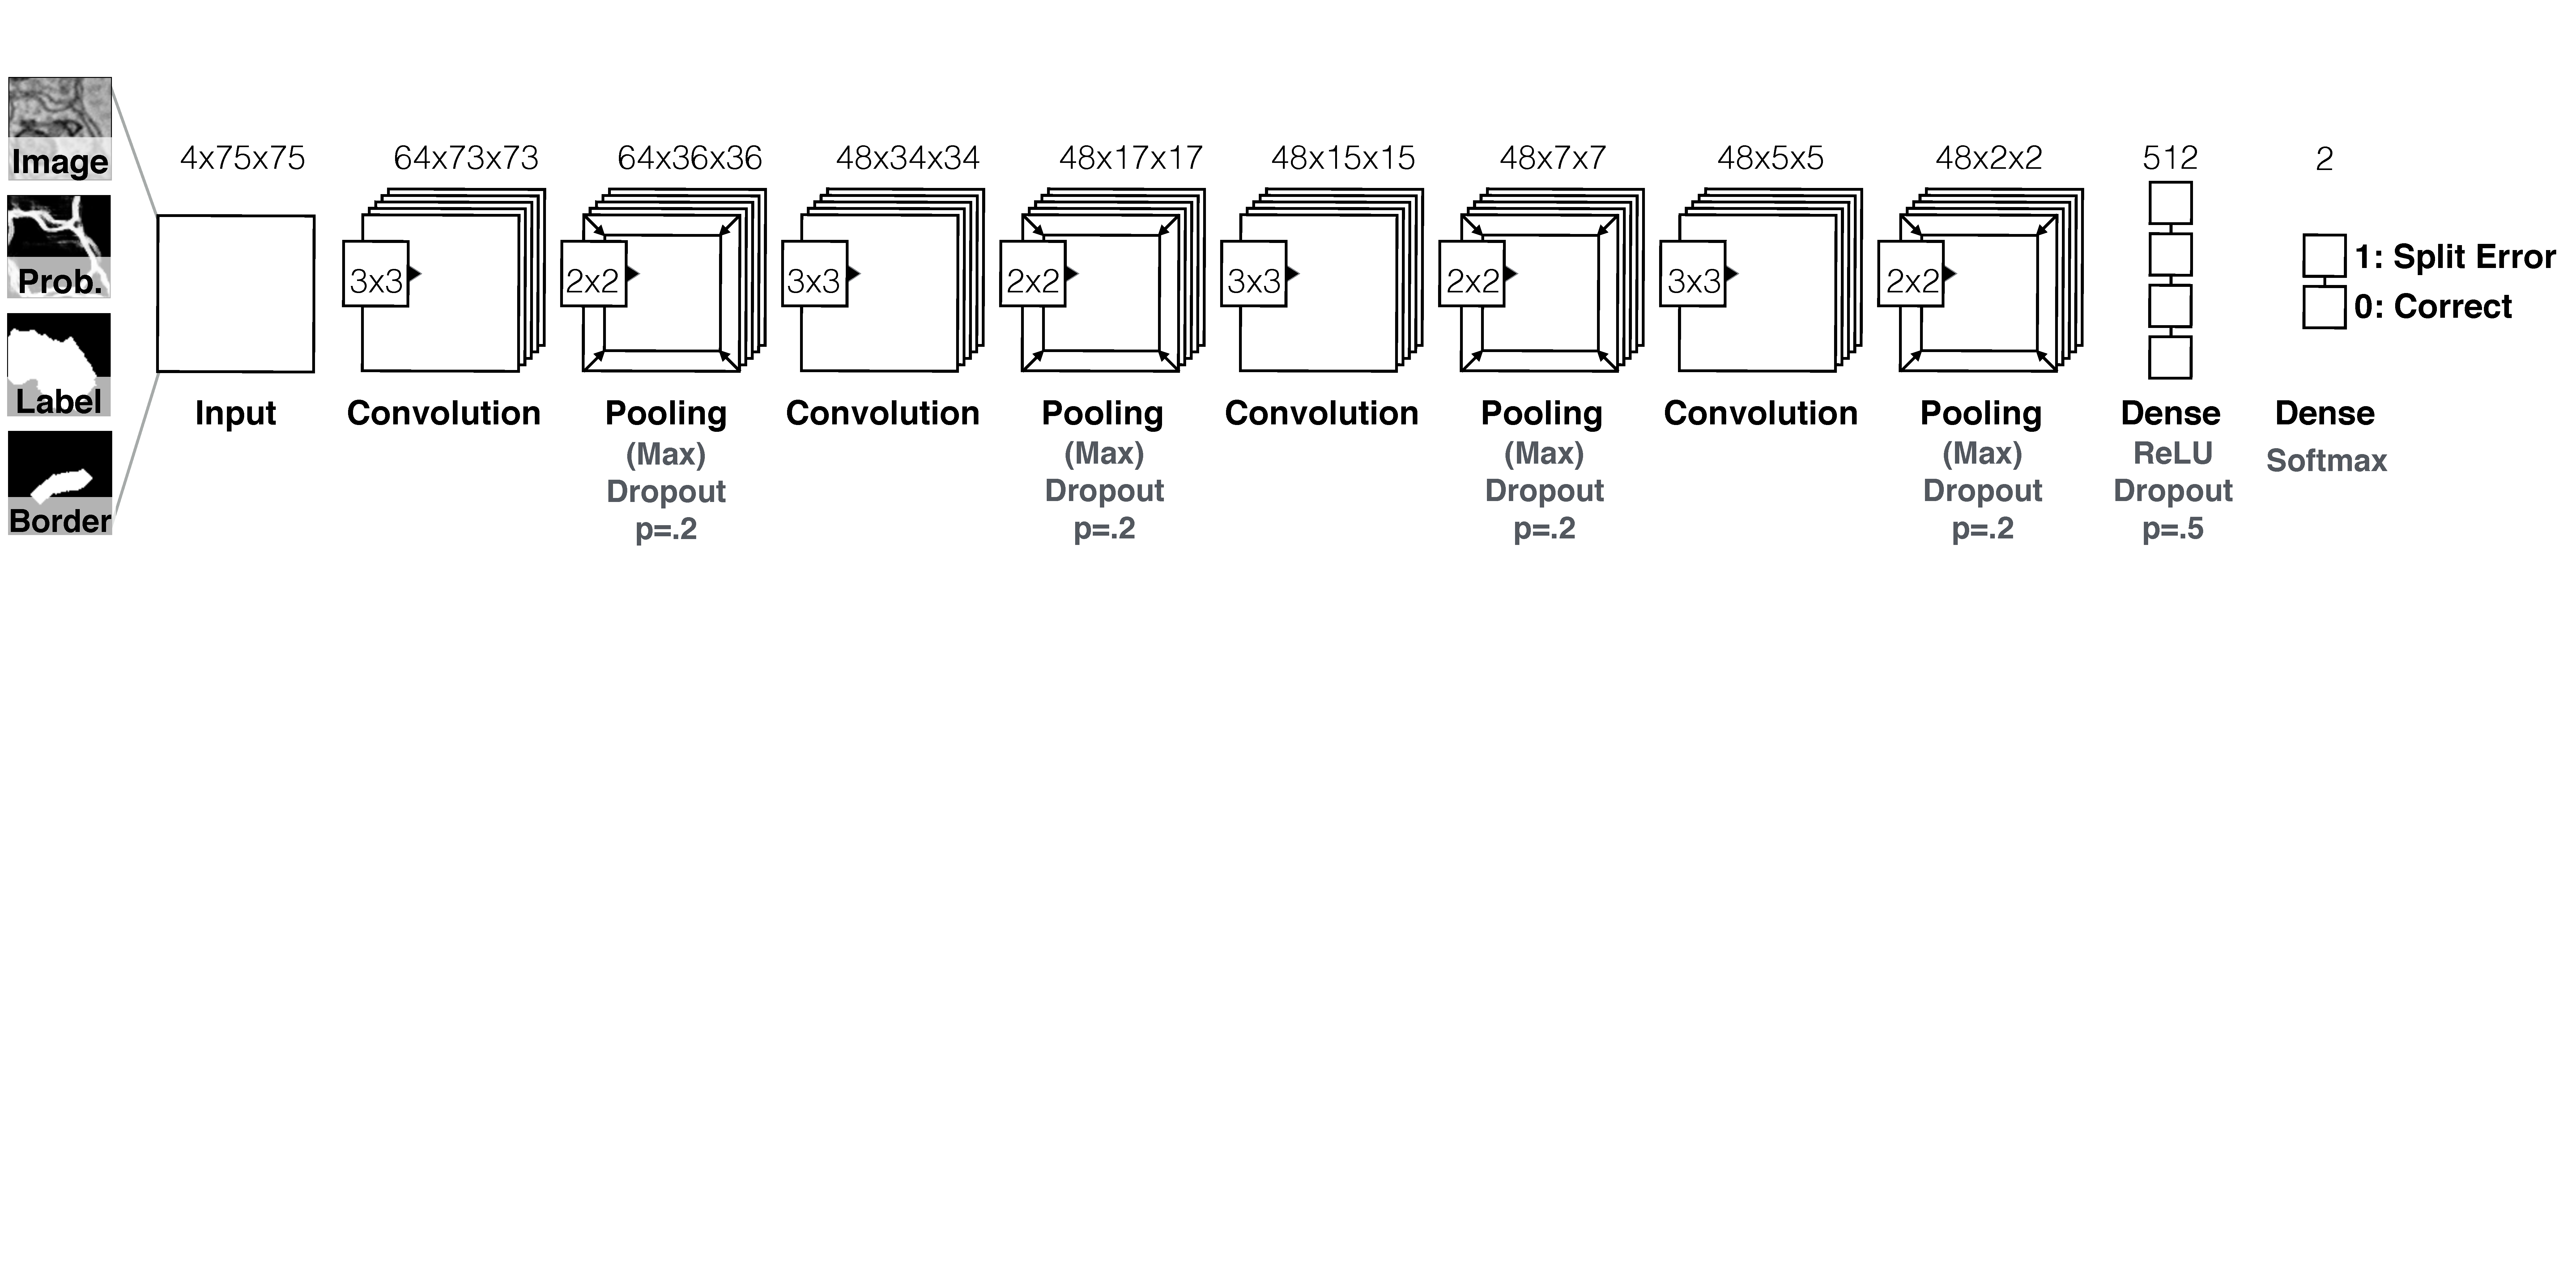
\includegraphics[width=\linewidth]{gfx/architecture.pdf}
\caption{Our guided proofreading classifiers use a traditional CNN architecture of four convolutional layers, each followed by max pooling and dropout regularization. The 4-channel input patches are labelled either as correct splits or as split errors.}
\label{fig:architecture}
\end{figure*}

\section{Related Work}

\textbf{Automatic Segmentation.} Multi-terabyte EM brain volumes require automatic segmentation~\cite{jain2010,Liu2014,NunezIglesias2013Machine,GALA2014}, but can be hard to classify due to ambiguous intercellular space: the 2013 IEEE ISBI neurites 3D segmentation challenge~\cite{isbi_challenge} showed that existing algorithms that learn from expert-segmented training data still exhibit high error rates.

Many works tackle this problem. NeuroProof~\cite{neuroproof2013} decreases error rates by learning an agglomeration on over-segmentations of images based on a random forest classifier. Vazquez-Reina \etal~\cite{amelio_segmentation} consider whole EM volumes rather than a per-section approach, then solve a fusion problem with a global context. Kaynig \etal~\cite{kaynig10} propose a random forest classifier coupled with an anisotropic smoothing prior in a conditional random field framework with 3D segment fusion. Bogovic \etal~\cite{BogovicHJ13} learn 3D features unsupervised, and show that they can be better than by-hand designs.

It is also possible to learn segmentation classification features directly from images with CNNs. Ronneberger \etal~\cite{RonnebergerFB15} use a contracting/expanding CNN path architecture to enable precise boundary localization with small amounts of training data. Lee \etal~\cite{lee2015recursive} recursively train very deep networks with 2D and 3D filters to detect boundaries.
%
All these approaches make good progress; however, in general, proofreading is still required to correct errors.

\paragraph{Interactive Proofreading.} While proofreading is very time consuming, it is fairly easy for humans to perform corrections through splitting and merging segments. One expert tool is Raveler, introduced by Chklovskii~\etal~\cite{chklovskii2010, raveler}. Raveler is used today by professional proofreaders, and it offers many parameters for tweaking the process. Similar systems exist as products or plugins to visualization systems,~\eg, V3D~\cite{proofreading_bottleneck} and AVIZO~\cite{markus_proofreading}.

Recent papers have attacked the problem of proofreading massive datasets through crowdsourcing with novices~\cite{saalfeld09,anderson2011,Giuly2013DP2}. One popular platform is EyeWire, by Kim \etal~\cite{eyewire_nature}, where participants earn virtual rewards for merging over-segmented labelings to reconstruct retina cells.

Between expert systems and online games sit Mojo and Dojo, by Haehn
\etal~\cite{haehn_dojo_2014,Neuroblocks}, which use simple scribble interfaces
for error correction. Dojo extends this to distributed proofreading via a
minimalistic web-based user interface. The authors define requirements for
general proofreading tools, and then evaluate the accuracy and speed of Raveler,
Mojo, and Dojo through a quantitative user study (Sec.~3 and
4, ~\cite{haehn_dojo_2014}). Dojo had the highest performance. In this paper, we
use Dojo as a baseline for interactive proofreading.

All interactive proofreading solutions require the user to find potential errors manually, which takes the majority of the time~\cite{proofreading_bottleneck,haehn_dojo_2014}. Recent papers propose computer-aided proofreading systems to quicken this visual search task.

\paragraph{Computer-aided Proofreading.} Uzunbas \etal~\cite{uzunbas} showed that potential labeling errors can be found by considering the merge tree of an automatic segmentation method. The authors track uncertainty throughout the automatic labeling by training a conditional random field. This segmentation technique produces uncertainty estimates, which inform potential regions for proofreading to the user. While this applies to isotropic volumes, more work is needed to apply it to the typically anisotropic connectromics dataset volumes.

%Their method requires further work to overcome the requirement of isotropic volumes, a property not given for most connectomics datasets. Our approach, guided proofreading, works on isotropic as well as anisotropic data, and finds merge and split errors.

Karimov \etal~\cite{karimov_guided_volume_editing} propose guided volume editing, which measures the difference in histogram distributions in image data to find potential split and merge errors in the corresponding segmentation. This lets expert users correct labeled computer-tomography datasets, using several interactions per correction. To correct merge errors, the authors create a large number of superpixels within a single segment and then successively group them based on dissimilarities. We were inspired by this approach, but instead we generate single watershed boundaries to handle the intracellular variance in high-resolution EM images (Sec.~\ref{sec:methods}).

Most closely related to our approach is the work of
Plaza~\cite{focused_proofreading}, who proposed \textit{focused proofreading}.
This method generates affinity scores by analyzing a region adjacency graph
across slices, then finds the largest affinities based on a defined impact
score. This yields edges of potential split errors which can be presented to the
proofreader. Plaza reports that additional manual work is required to find and
correct merge errors. Focused proofreading builds upon
NeuroProof~\cite{neuroproof2013} as its agglomerator, and is open source with
integration into Raveler. As the closest related work, we wish to use this
method as a baseline to evaluate our approach (Sec.~\ref{sec:evaluation}).
However, we separate the backend affinity score calculation from the Raveler
expert-level front end, and present our own novice-friendly interface
(Sec.~\ref{sec:evaluation}).
